\documentclass[11pt]{article}

\usepackage[margin=1in]{geometry}
\usepackage[T1]{fontenc}
\usepackage[utf8]{inputenc}
\usepackage{lmodern}
\usepackage{microtype}
\usepackage{amsmath}
\usepackage{amssymb}
\usepackage{array}
\usepackage{booktabs}
\usepackage{graphicx}
\usepackage{subcaption}
\usepackage{float}
\usepackage{xcolor}
\usepackage{siunitx}
\usepackage{orcidlink}
\usepackage{hyperref}
\usepackage[nameinlink,noabbrev]{cleveref}

\graphicspath{{figures/}}

\hypersetup{
  colorlinks=true,
  linkcolor=blue,
  citecolor=blue,
  urlcolor=blue
}

\sisetup{
  detect-all,
  separate-uncertainty=true
}

% V2 review highlighting; supports page breaks.
\usepackage{mdframed}

\newcommand{\dft}{\mathrm{DFT}}
\newcommand{\xtb}{\mathrm{xTB}}
\newcommand{\boe}{\mathrm{BoE}}
\newcommand{\pre}{\mathrm{PRE}}
\newcommand{\gemnet}{\mathrm{GemNet}}
\newcommand{\qmNine}{\mathrm{QM9}}
\newcommand{\tmqm}{\mathrm{tmQM}}
\newcommand{\target}{y}
\newcommand{\baseline}{b}
\newcommand{\residual}{r}
\newcommand{\prediction}{\hat{y}}
\newcommand{\mae}{\mathrm{MAE}}
\newcommand{\rTwo}{R^2}

\usepackage{float}

\renewcommand{\thefigure}{S\arabic{figure}}
\renewcommand{\thetable}{S\arabic{table}}

\title{Supplementary Information for\\
Beyond Variance Reduction: Target Design for Generalizable Machine-Learning Interatomic Potentials}
\author{
  \orcidlink{0000-0002-1168-9830}\hspace{1mm}Kareem M.~Gameel\\
  Department of Physical and Environmental Sciences, University of Toronto Scarborough\\
  Alliance for AI-Accelerated Materials Discovery (A3MD)\\
  Toronto, Ontario, Canada
  \and
  \orcidlink{0000-0001-9906-8010}\hspace{1mm}Ihor Neporozhnii\\
  Department of Physical and Environmental Sciences, University of Toronto Scarborough\\
  Alliance for AI-Accelerated Materials Discovery (A3MD)\\
  Toronto, Ontario, Canada
  \and
  \orcidlink{0000-0002-8656-5074}\hspace{1mm}Oleksandr Voznyy\\
  Department of Chemistry, University of Toronto\\
  Department of Physical and Environmental Sciences, University of Toronto Scarborough\\
  Alliance for AI-Accelerated Materials Discovery (A3MD)\\
  Toronto, Ontario, Canada
}
\date{}

\begin{document}

\maketitle

\linenumbers

This Supplementary Information follows the order of the main manuscript. Short notes are included only where they clarify how a control figure should be interpreted; the primary discussion remains in the main text.

\section*{Supplementary Figures}

Figures~S1--S5 provide controls and architecture-level checks that support the main text without changing the central GemNet-focused narrative. Figure~S1 verifies full-target reconstruction after BoE preprocessing. Figures~S2--S5 document SchNet companion results, correlation controls, and ridge-versus-MLP descriptor-baseline controls.

\begin{figure}[H]
  \centering
  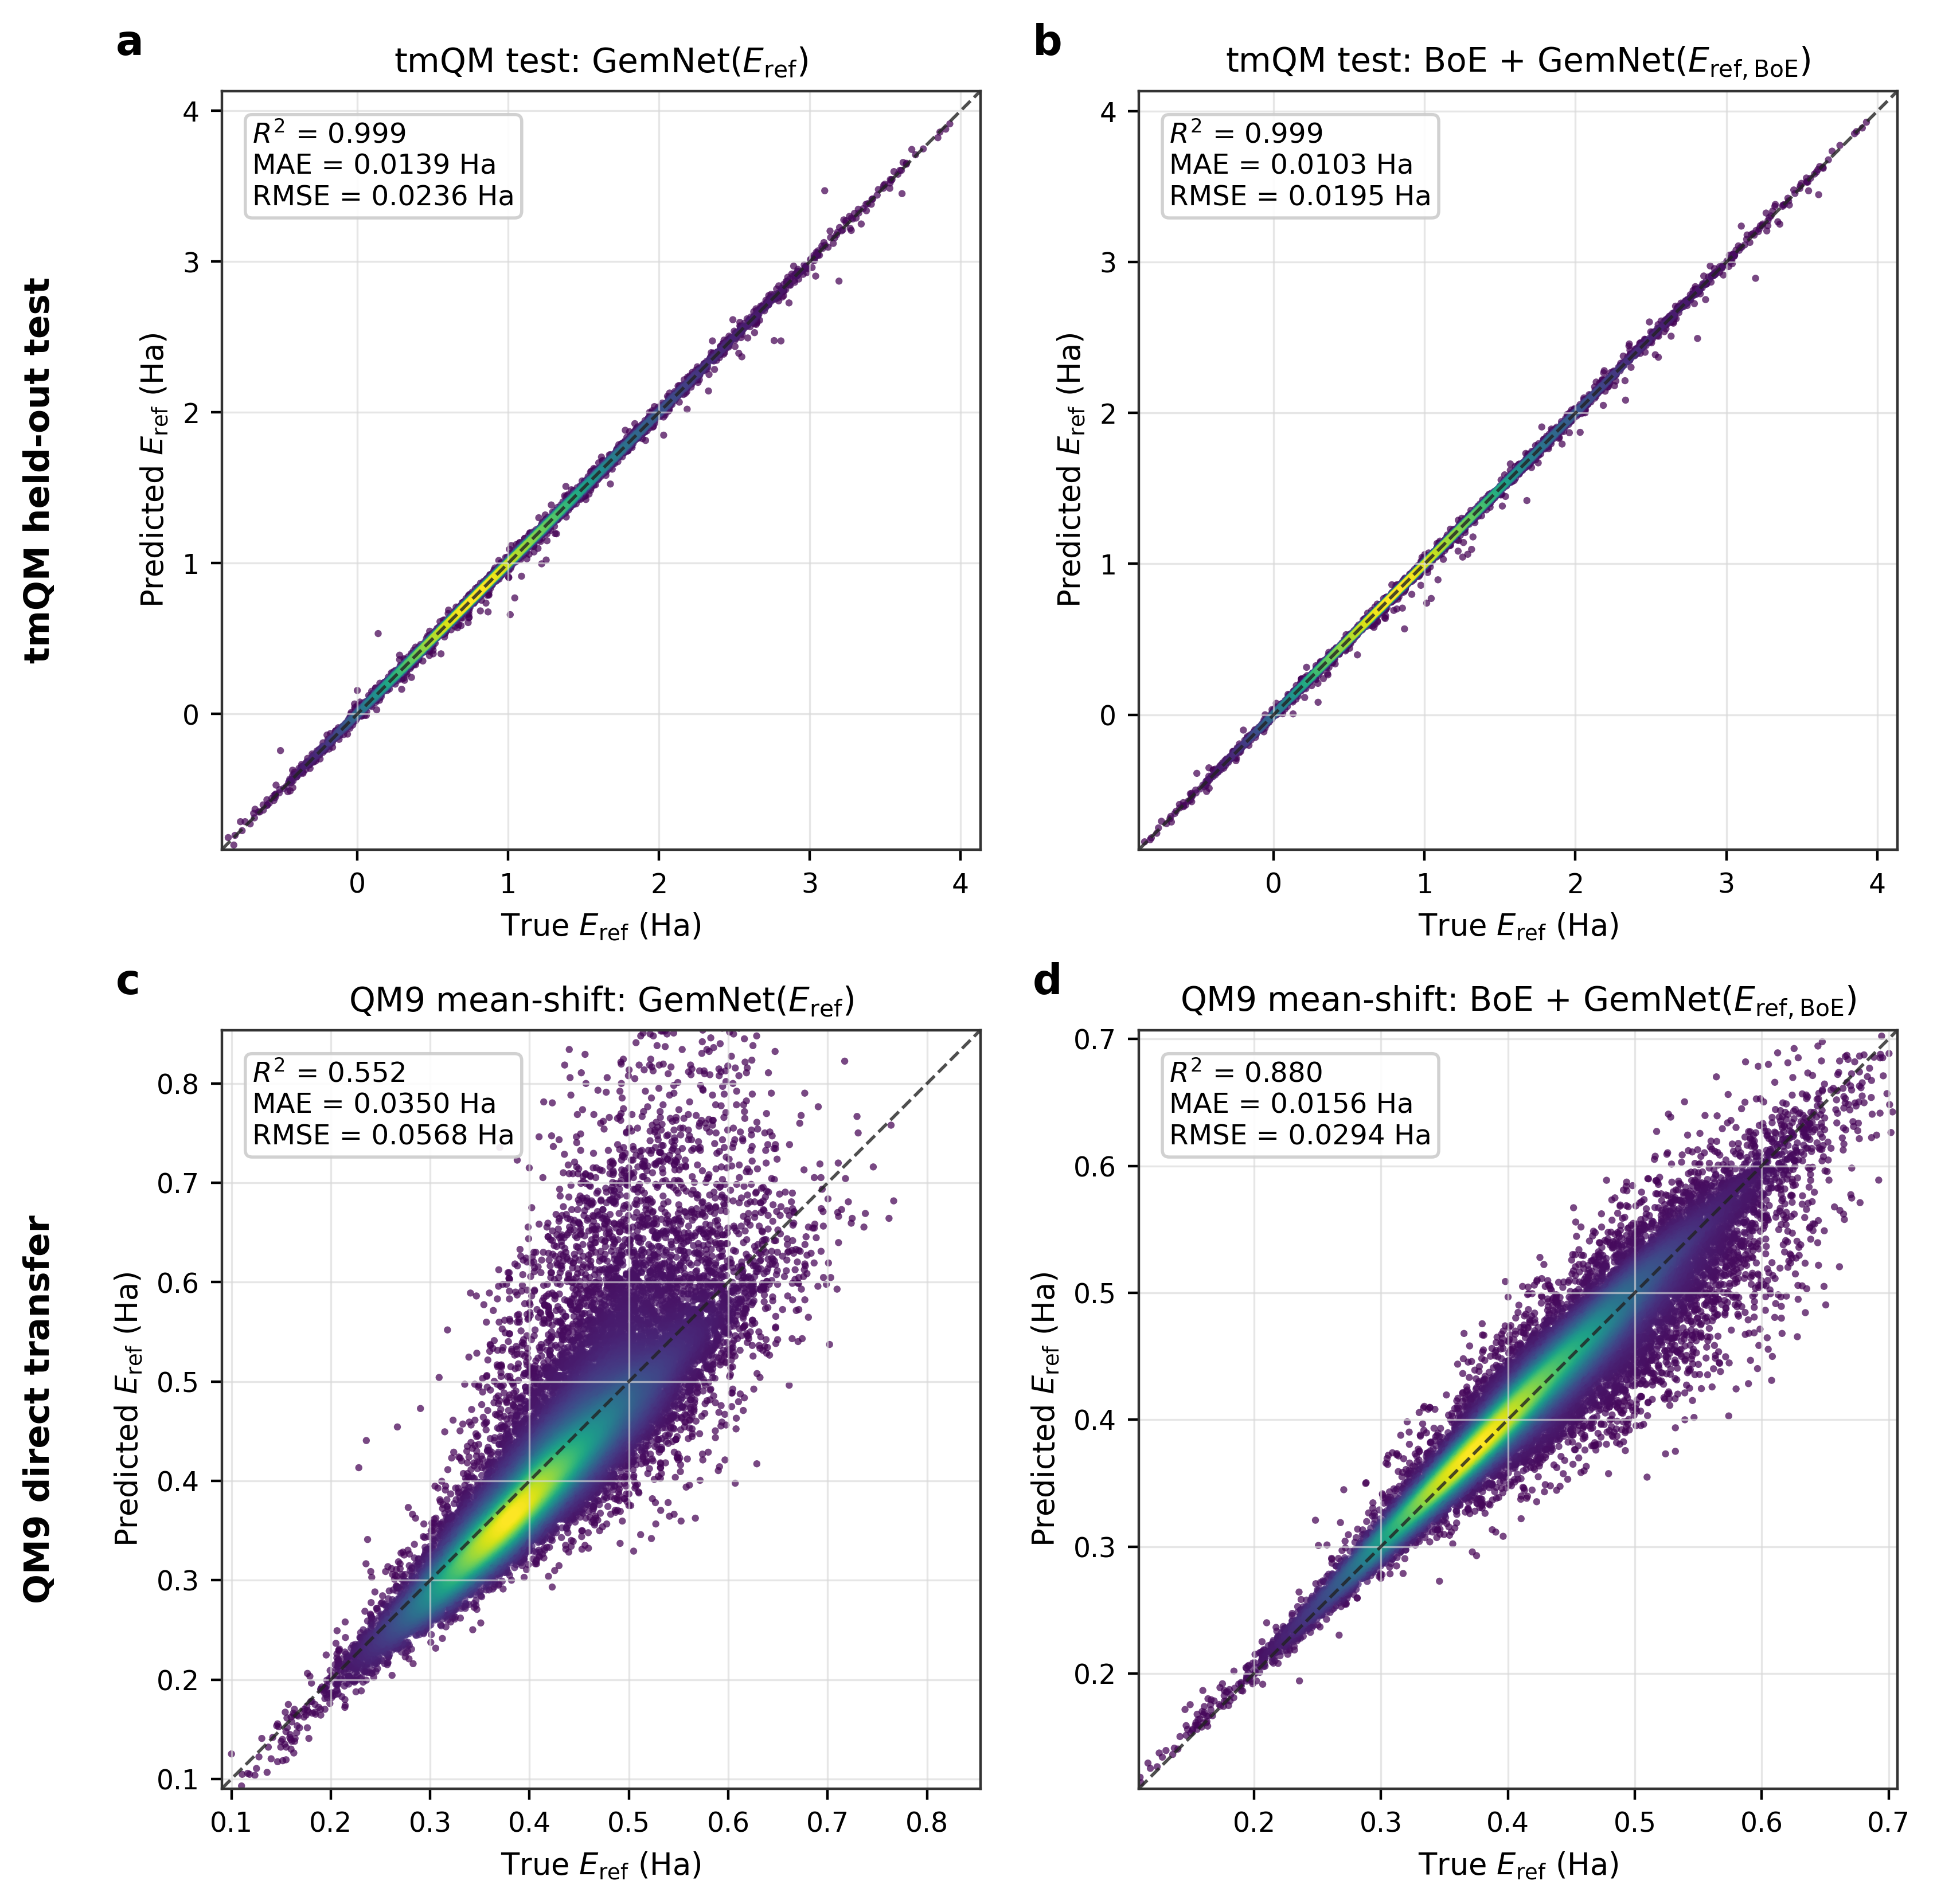
\includegraphics[width=0.95\linewidth]{fig_gemnet_dftref_vs_dftrefboe_parity}
  \caption{Effect of BoE target preprocessing on GemNet predictions evaluated on the same full-target scale. The top row shows held-out tmQM test predictions against \(E_{\rm ref}\). The bottom row shows direct transfer to QM9 after mean-shift calibration. For the BoE-preprocessed model, the plotted prediction is the reconstructed full target, \(E_{\rm BoE} + {\rm GemNet}(E_{\rm ref,BoE})\).}
  \label{fig:s1-gemnet-dftref-vs-dftrefboe-parity}
\end{figure}

\begin{figure}[H]
  \centering
  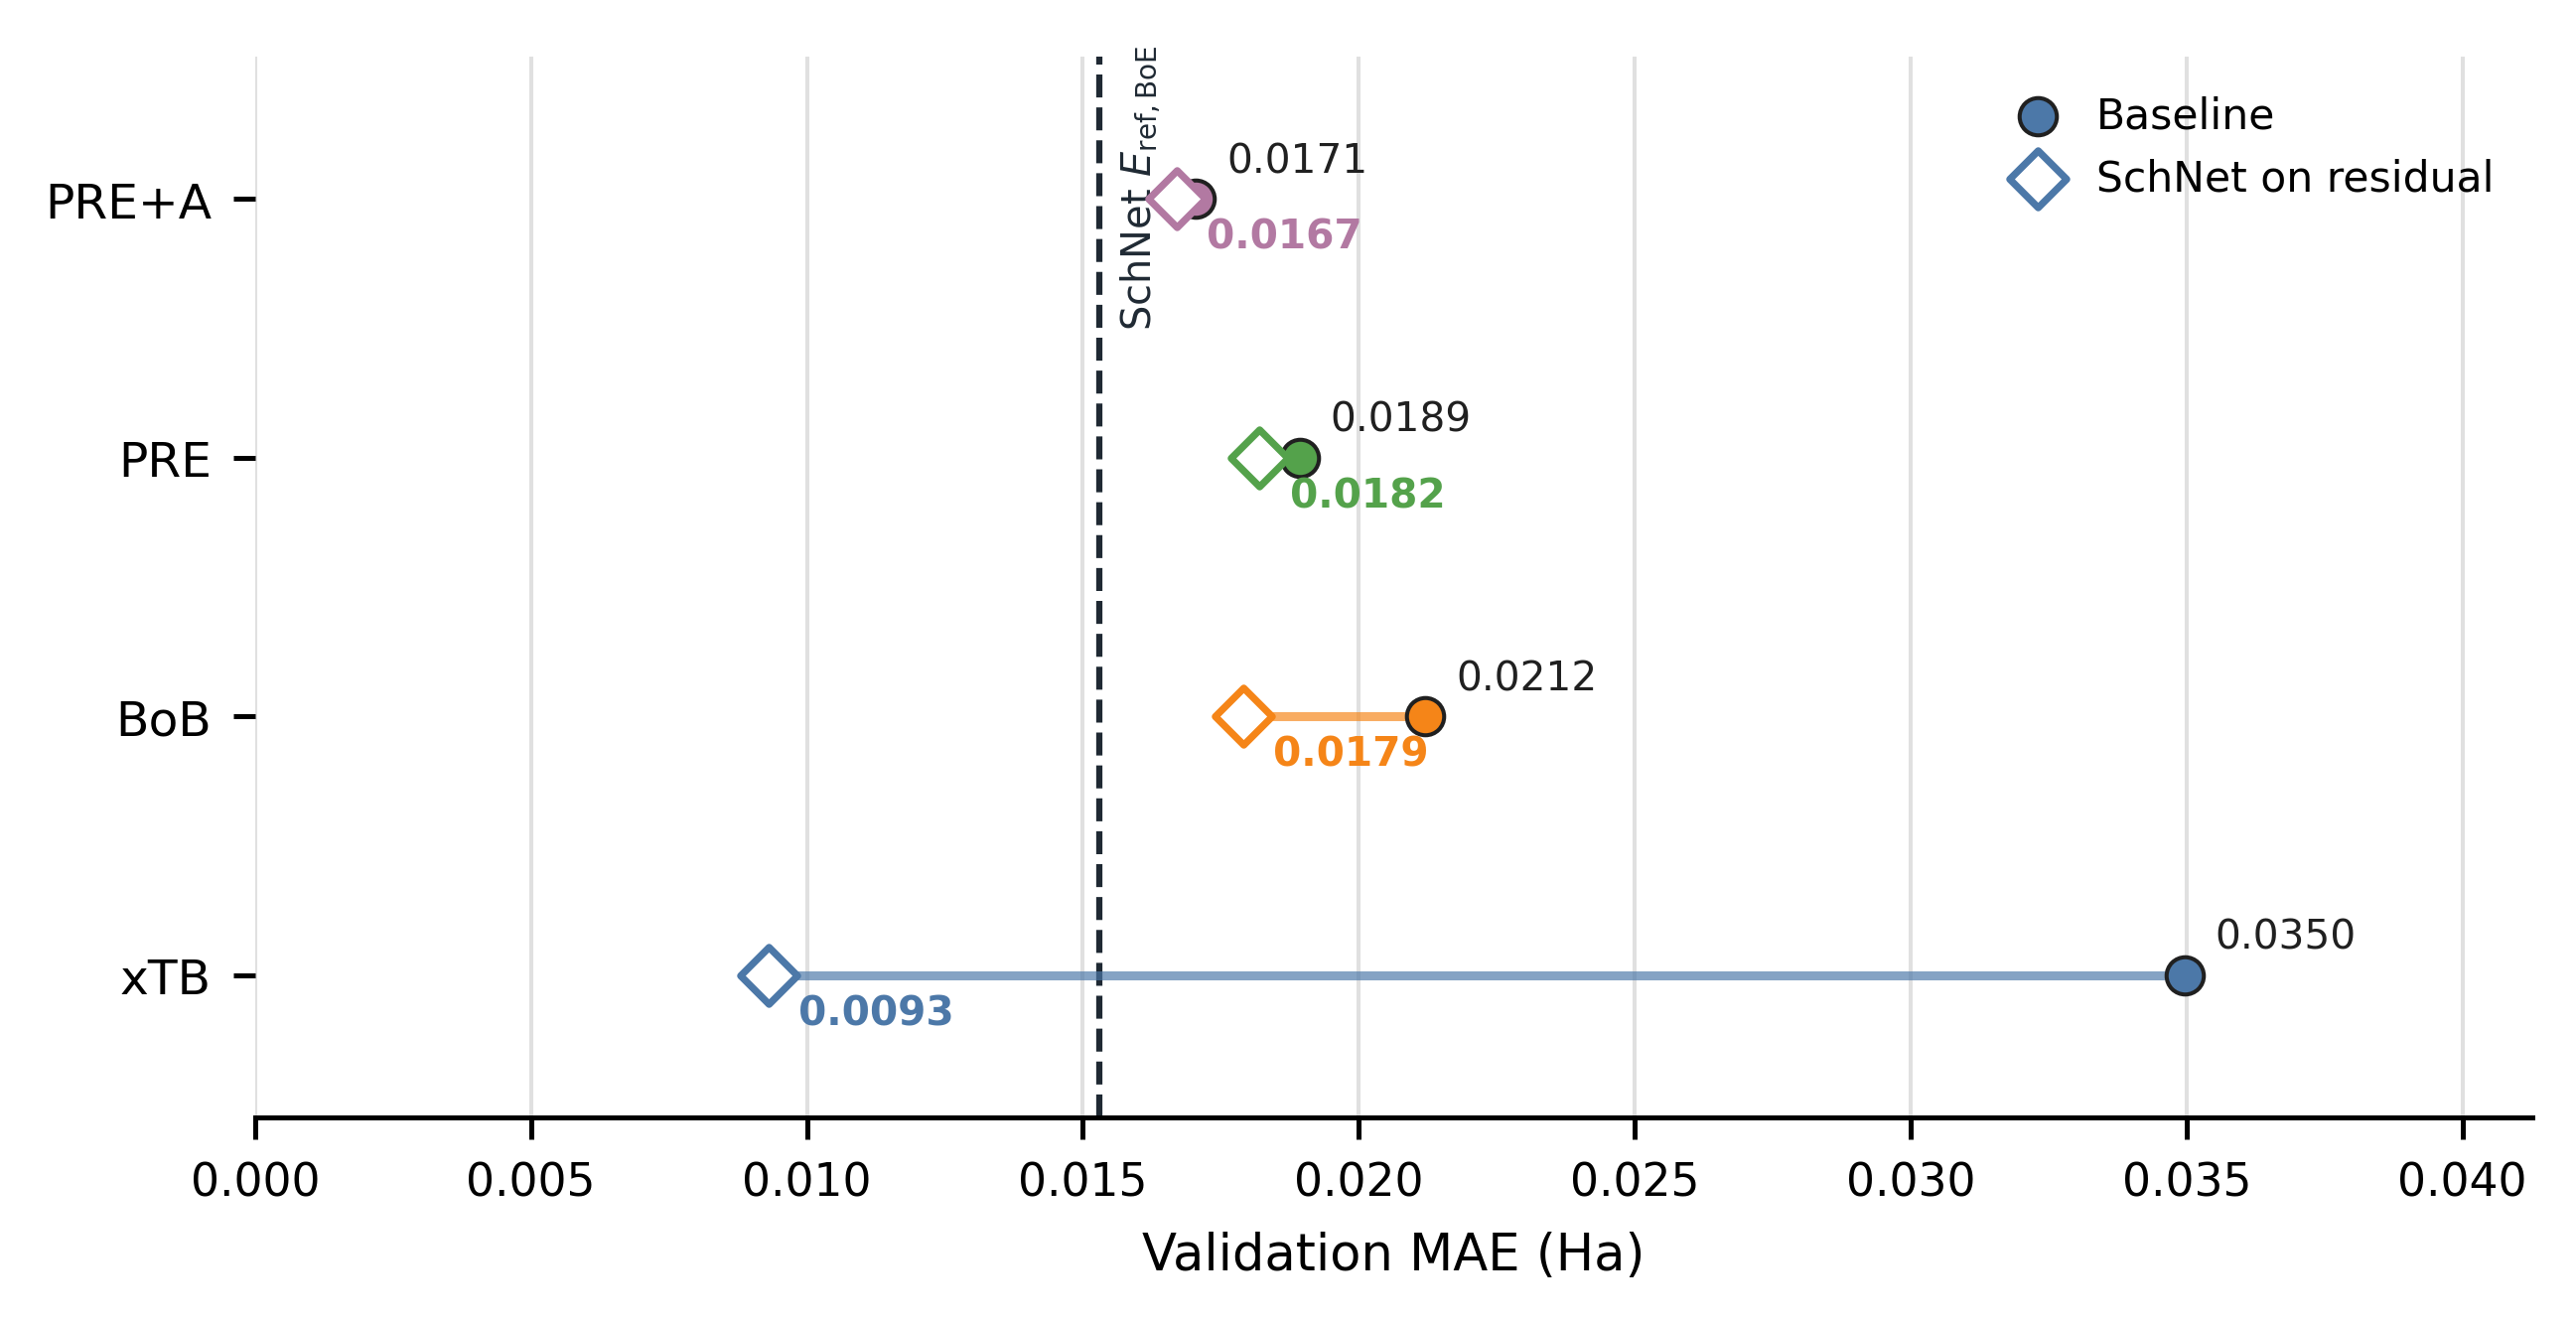
\includegraphics[width=0.95\linewidth]{baseline_to_schnet_residual_mae_cleveland}
  \caption{Residual-learning trend reproduced with SchNet. Filled circles show the validation MAE of each baseline on \(E_{\rm ref,BoE}\), and open diamonds show the reconstructed validation MAE after training SchNet on the corresponding residual target. The dashed vertical line marks direct SchNet training on \(E_{\rm ref,BoE}\) without residualization. All values are tmQM validation-set MAEs in Hartree using the same split.}
  \label{fig:s2-baseline-to-schnet-residual-mae}
\end{figure}

\begin{figure}[H]
  \centering
  \begin{subfigure}{0.49\linewidth}
    \centering
    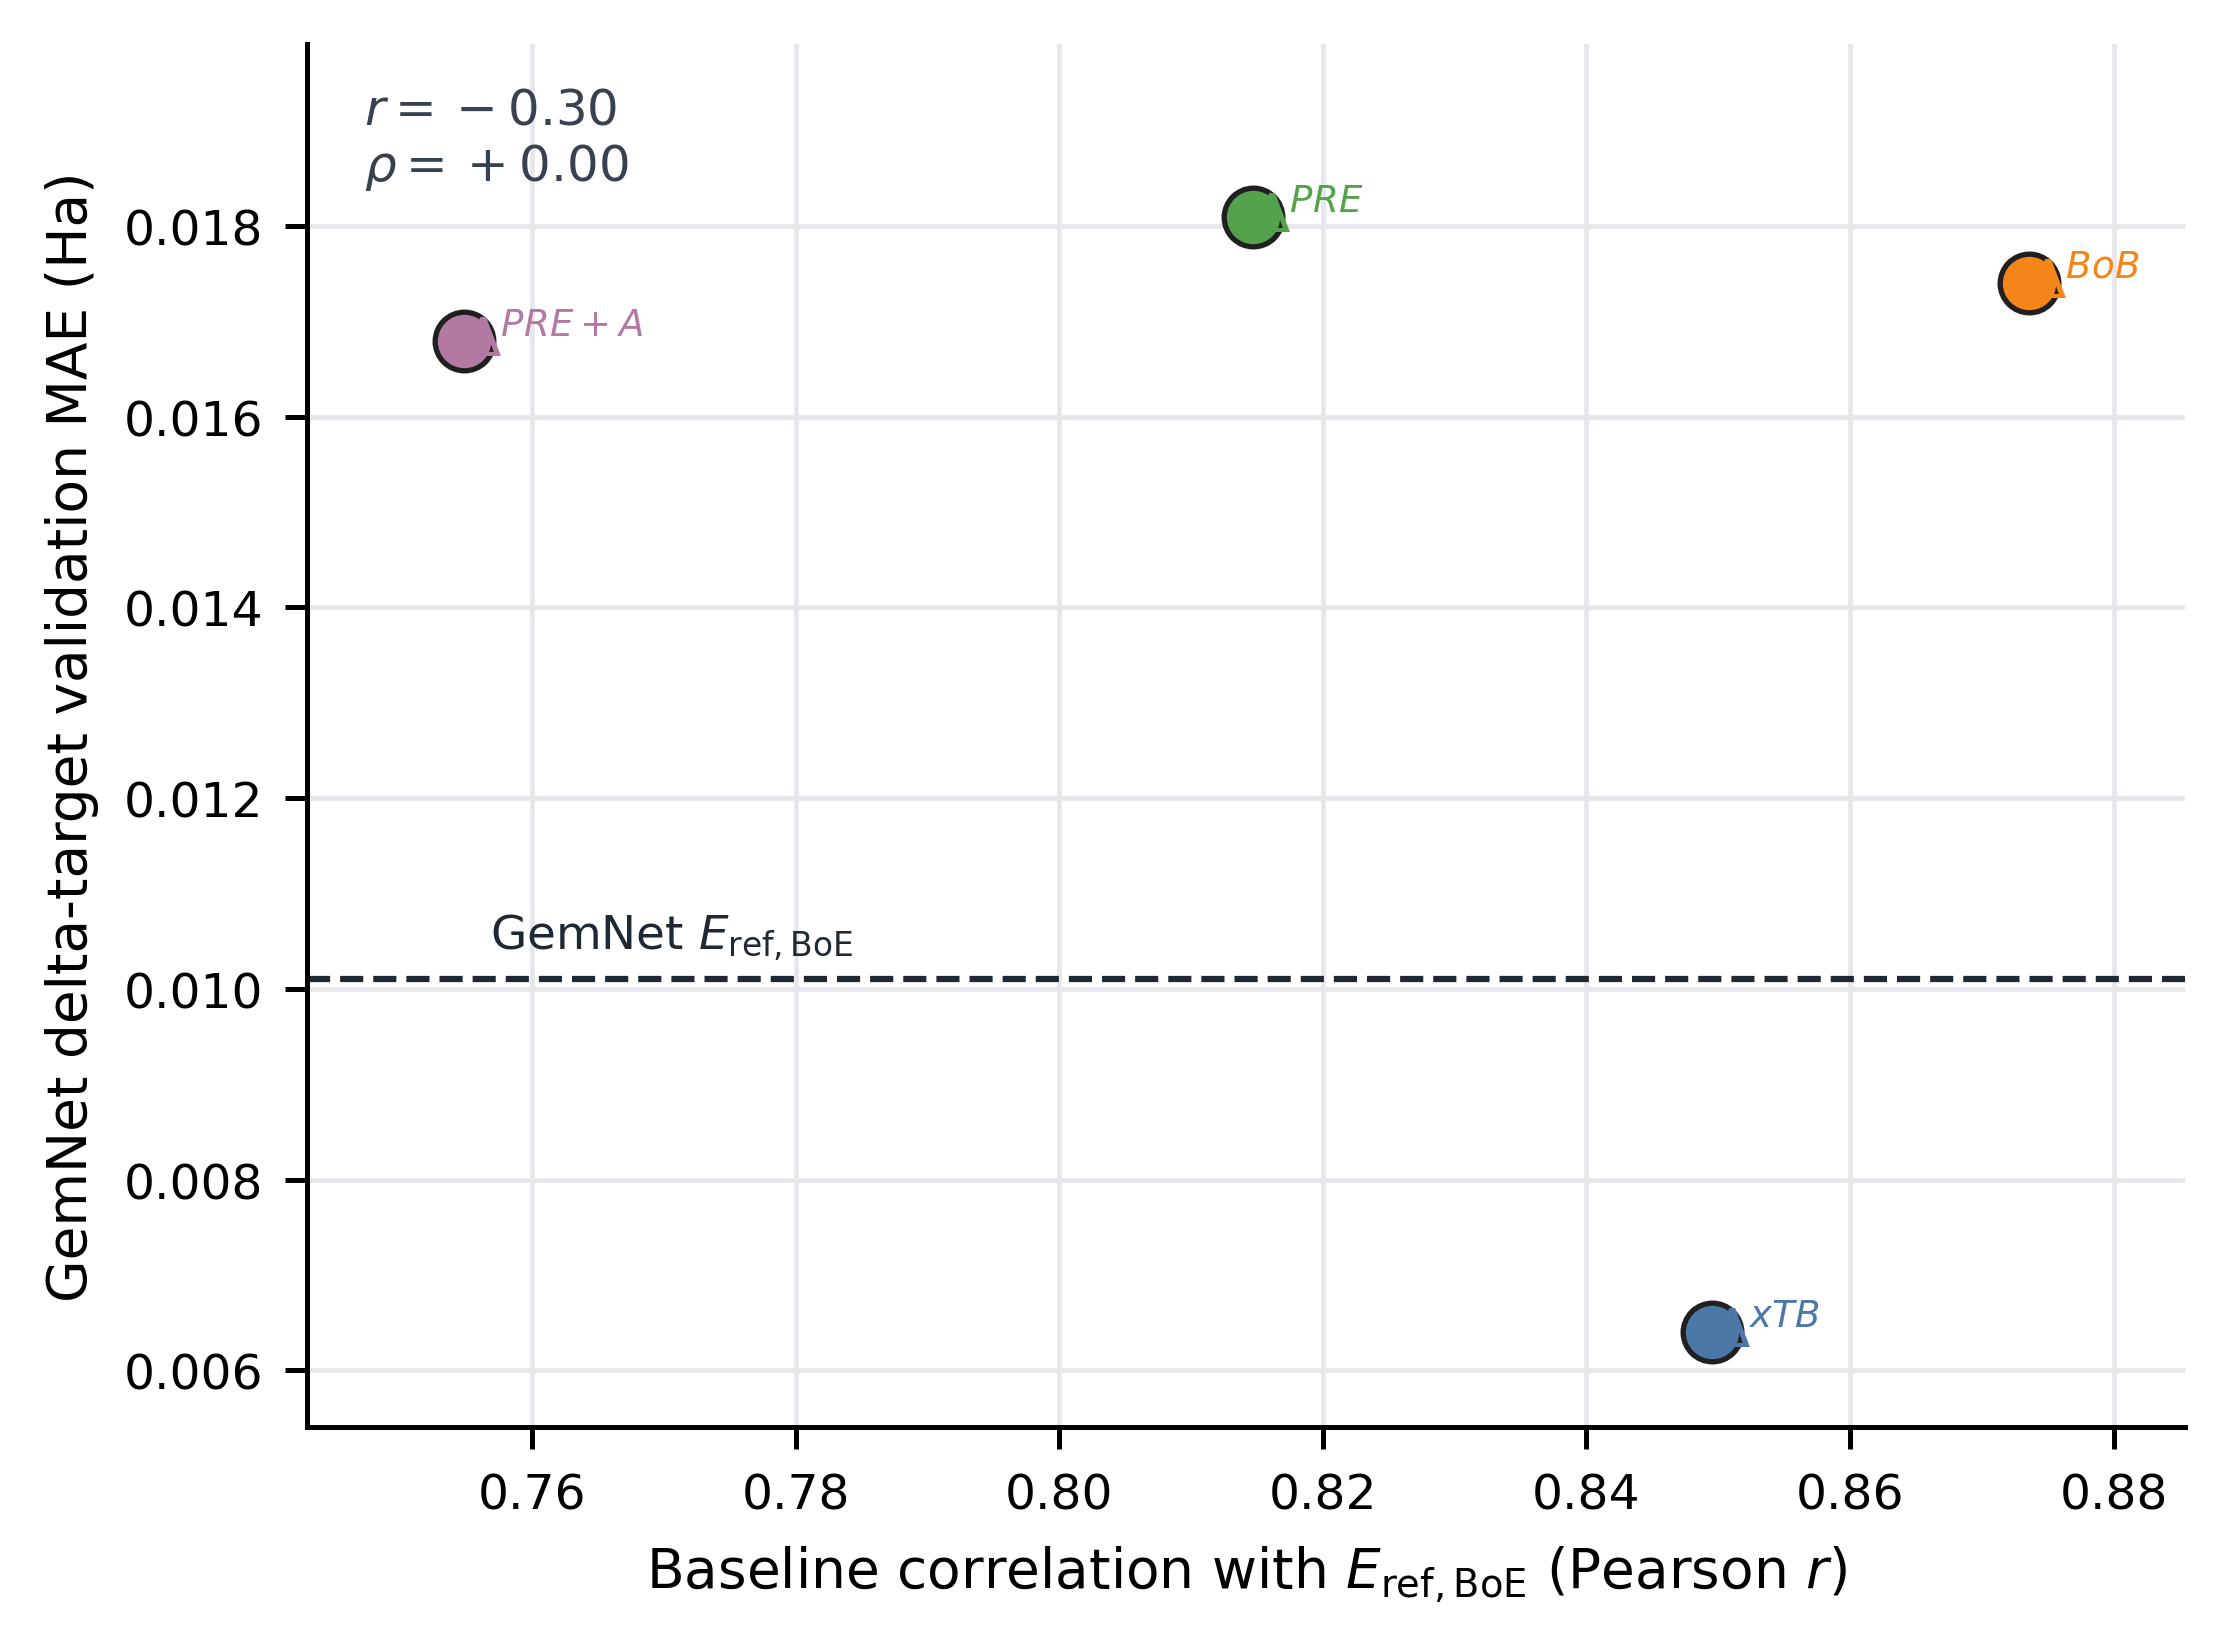
\includegraphics[width=\linewidth]{baseline_correlation_vs_gemnet_delta_mae}
    \caption{Pearson correlation.}
  \end{subfigure}
  \hfill
  \begin{subfigure}{0.49\linewidth}
    \centering
    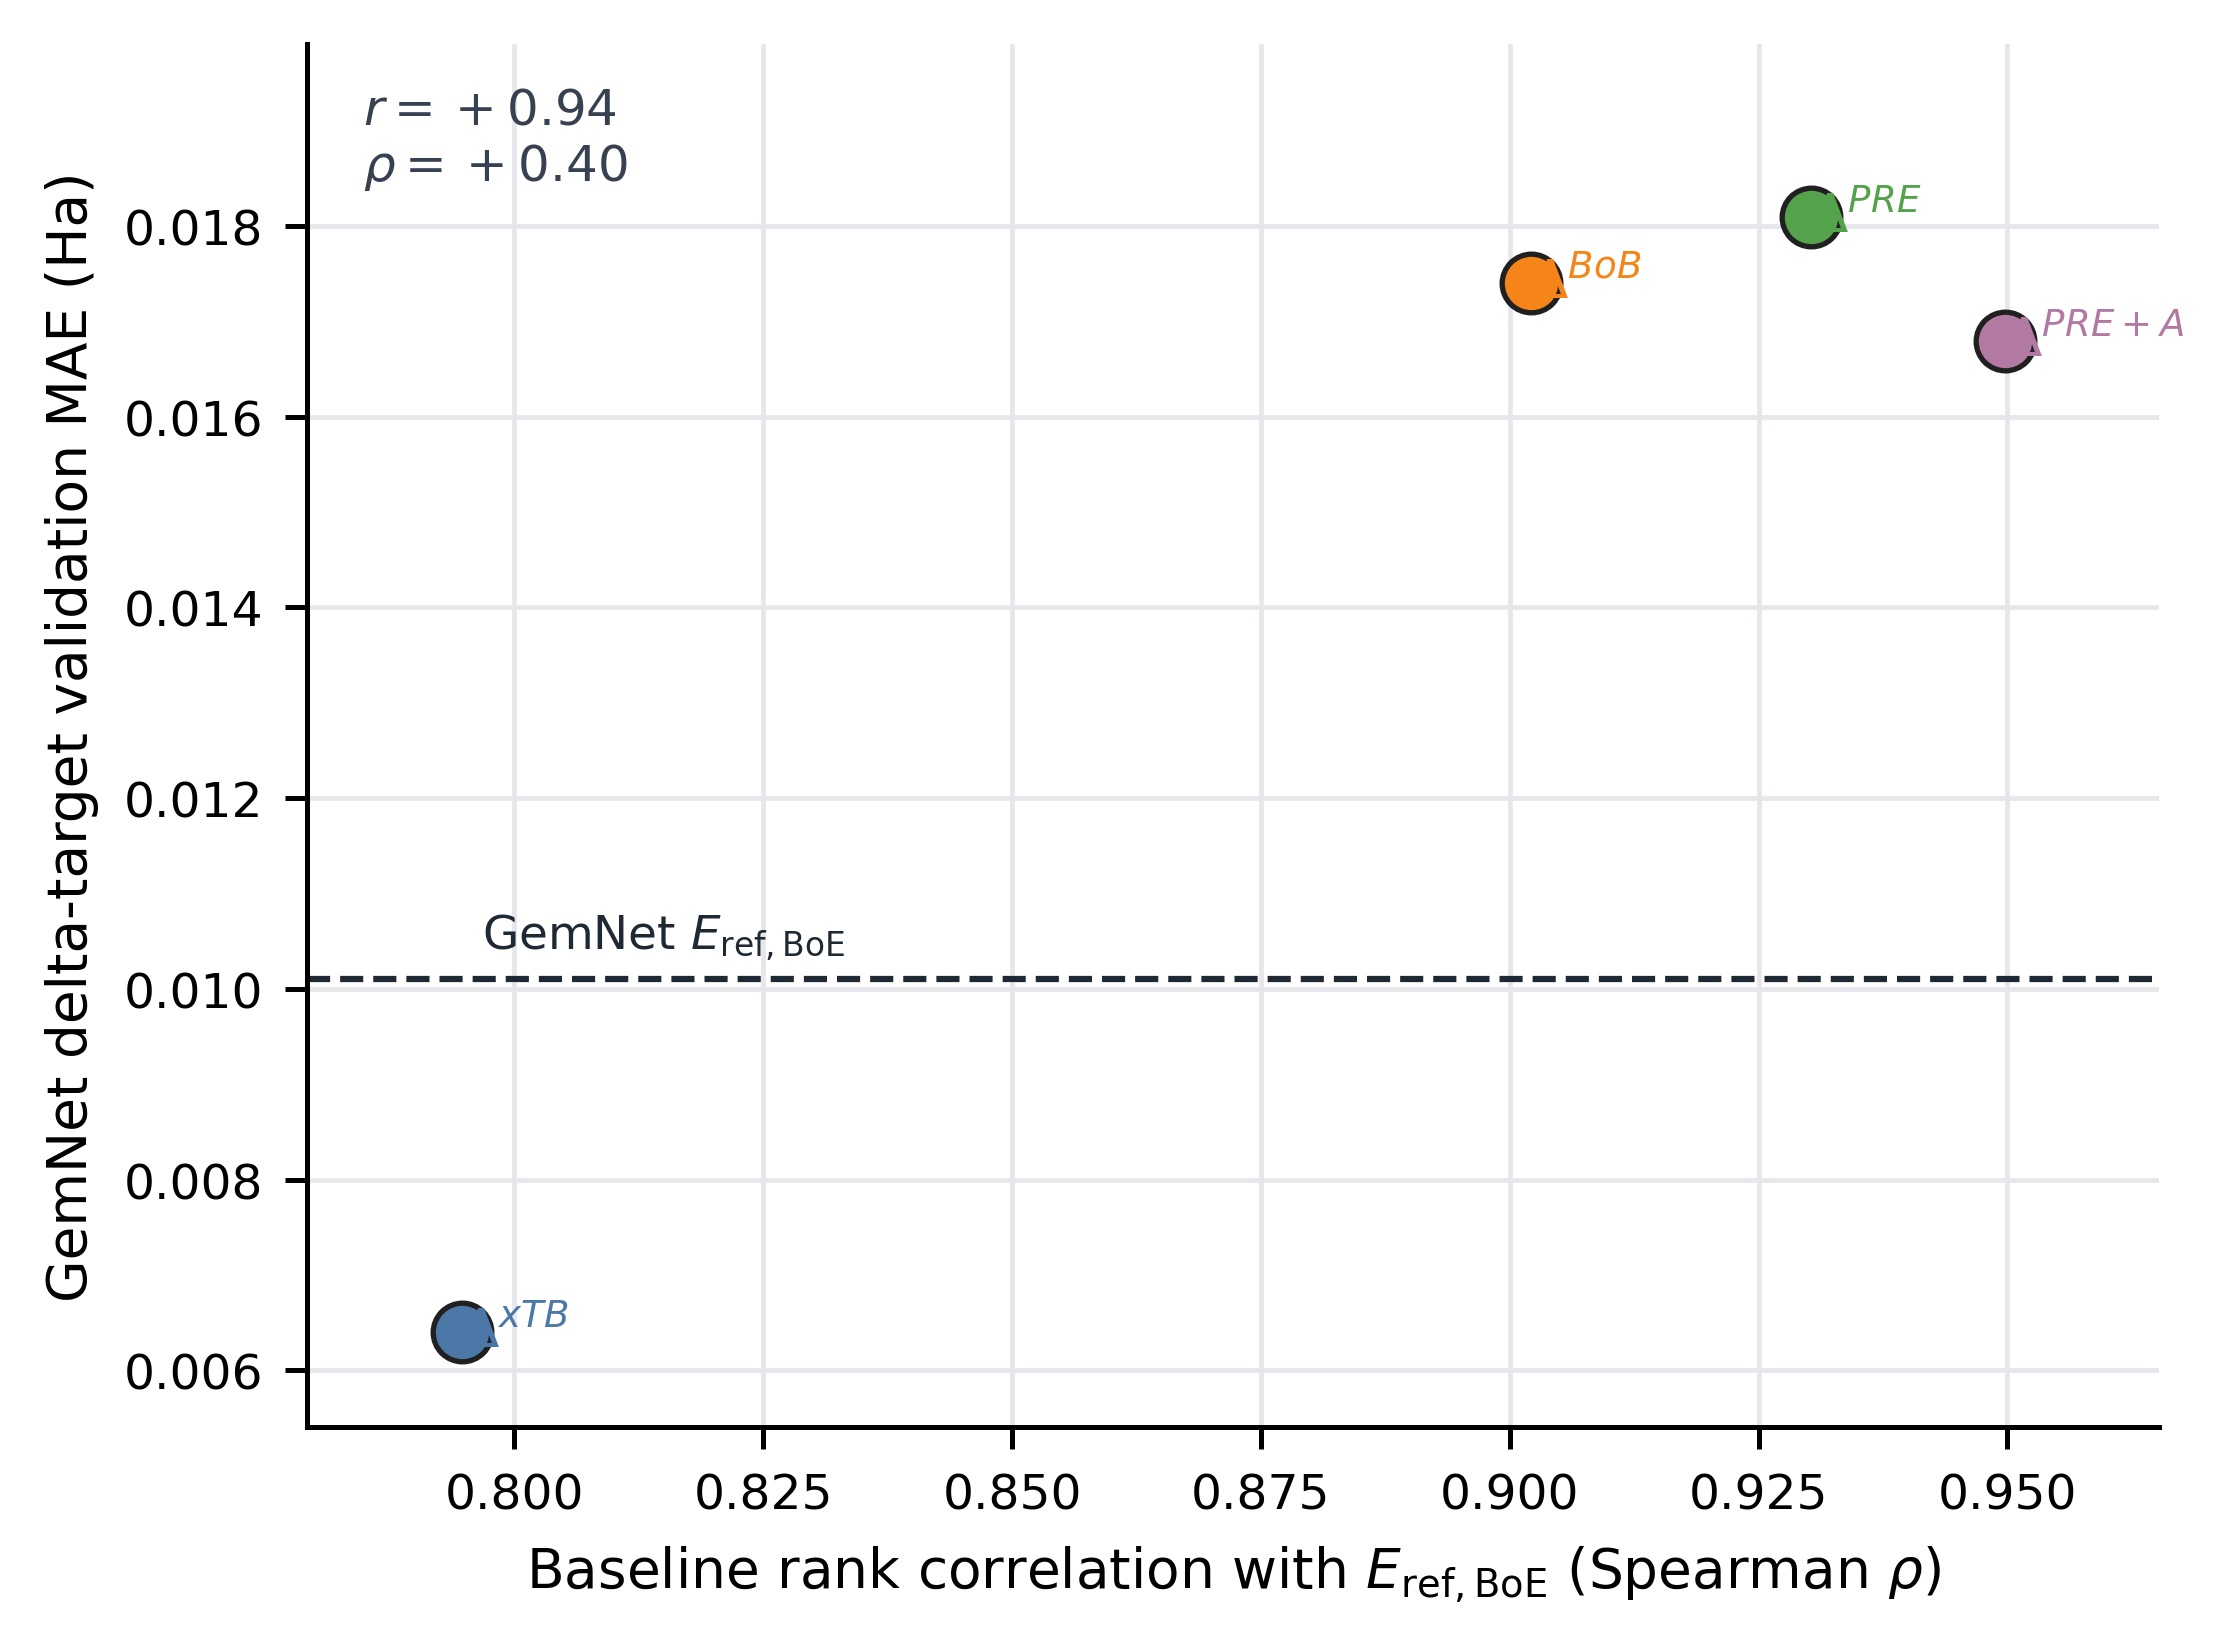
\includegraphics[width=\linewidth]{baseline_spearman_vs_gemnet_delta_mae}
    \caption{Spearman rank correlation.}
  \end{subfigure}
  \caption{Baseline-target correlation does not predict residual GemNet performance. Each point corresponds to one baseline used to construct a residual target from \(E_{\rm ref,BoE}\). The vertical axis reports the reconstructed GemNet validation MAE after residual learning. Although the descriptor baselines have stronger correlation with \(E_{\rm ref,BoE}\), xTB yields the lowest residual-learning error. The global correlation annotations should be interpreted qualitatively because the panel contains only four baselines.}
  \label{fig:s3-baseline-correlation-diagnostics}
\end{figure}

\begin{figure}[H]
  \centering
  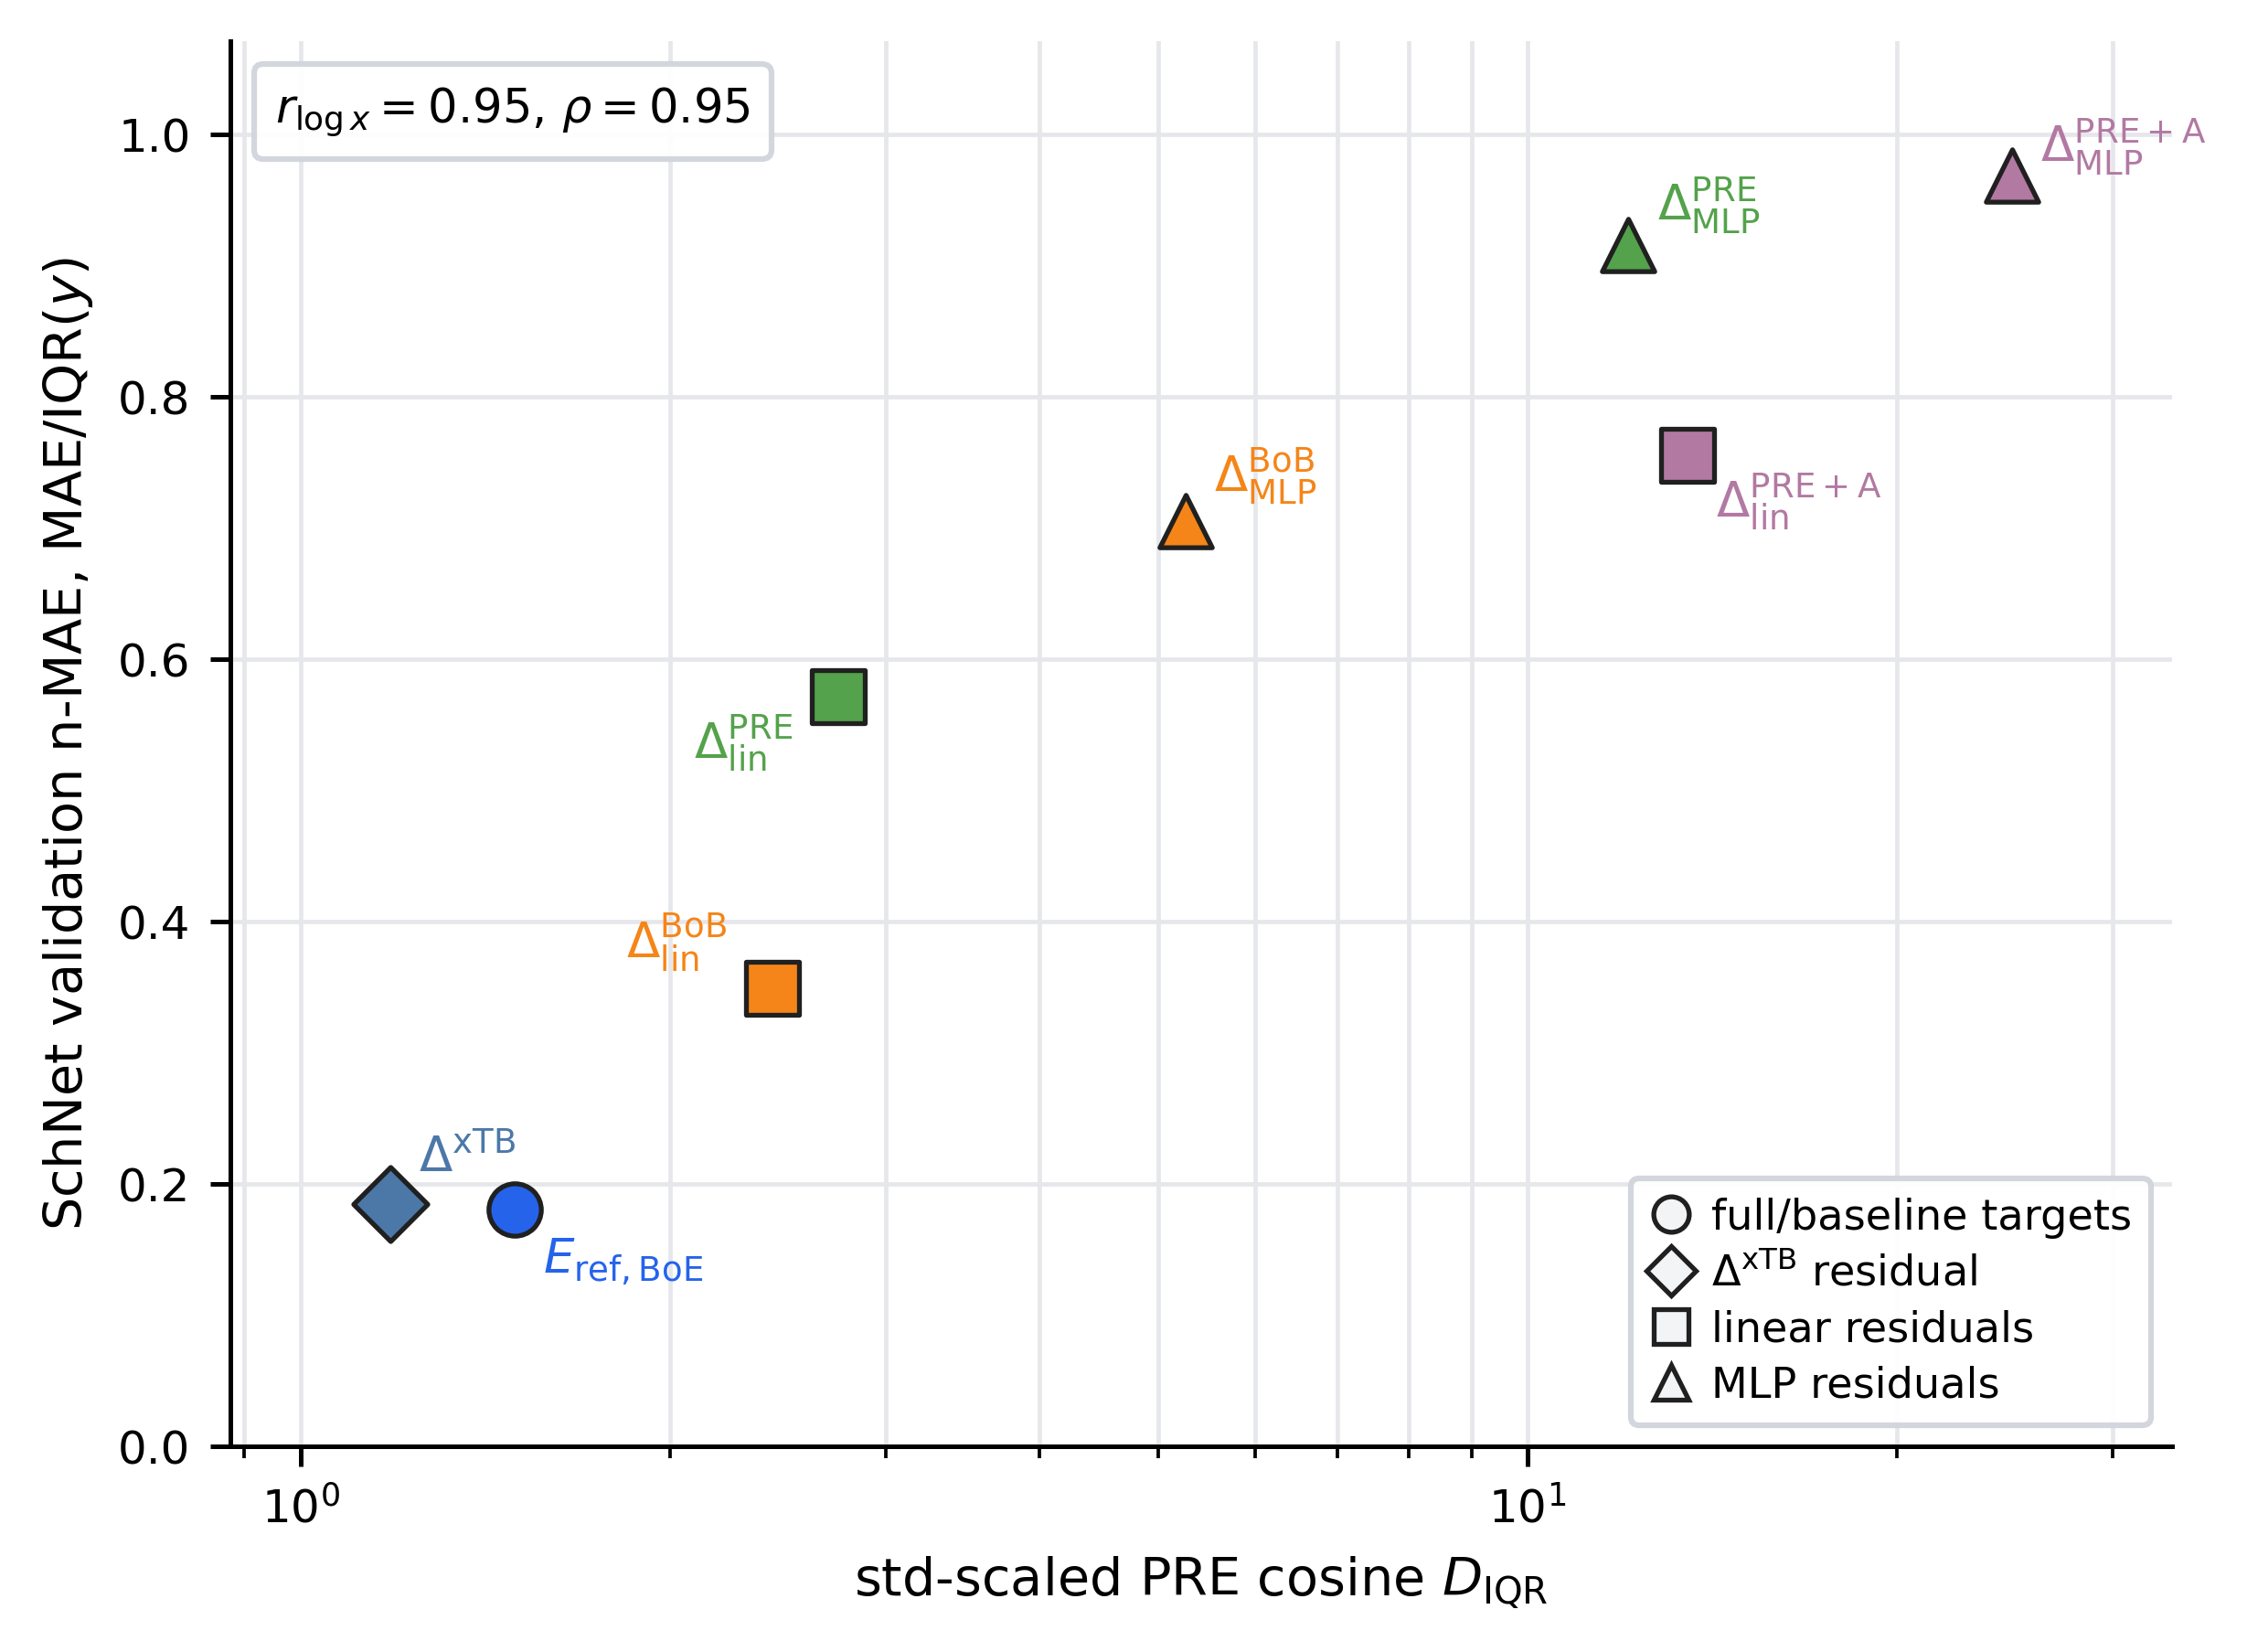
\includegraphics[width=0.95\linewidth]{schnet_iqr_nmae_vs_pre_std_iqr_norm_dirichlet_cosine_linear_mlp}
  \caption{SchNet companion to the GemNet roughness-learning diagnostic. The horizontal axis reports \(D_{\rm IQR}\), measured on a \(k=10\) cosine nearest-neighbor graph built from standardized PRE descriptors on the tmQM validation split. PRE is used as a pair-distance proxy for the information explicitly available to SchNet. The vertical axis reports SchNet validation \(n\)-MAE, defined as MAE divided by the target IQR. The available SchNet panel shows the same qualitative trend as GemNet: rougher residual targets in the model-aligned feature space have larger scale-normalized learning errors.}
  \label{fig:s4-baseline-to-residual-roughness-pre-space}
\end{figure}

\begin{figure}[H]
  \centering
  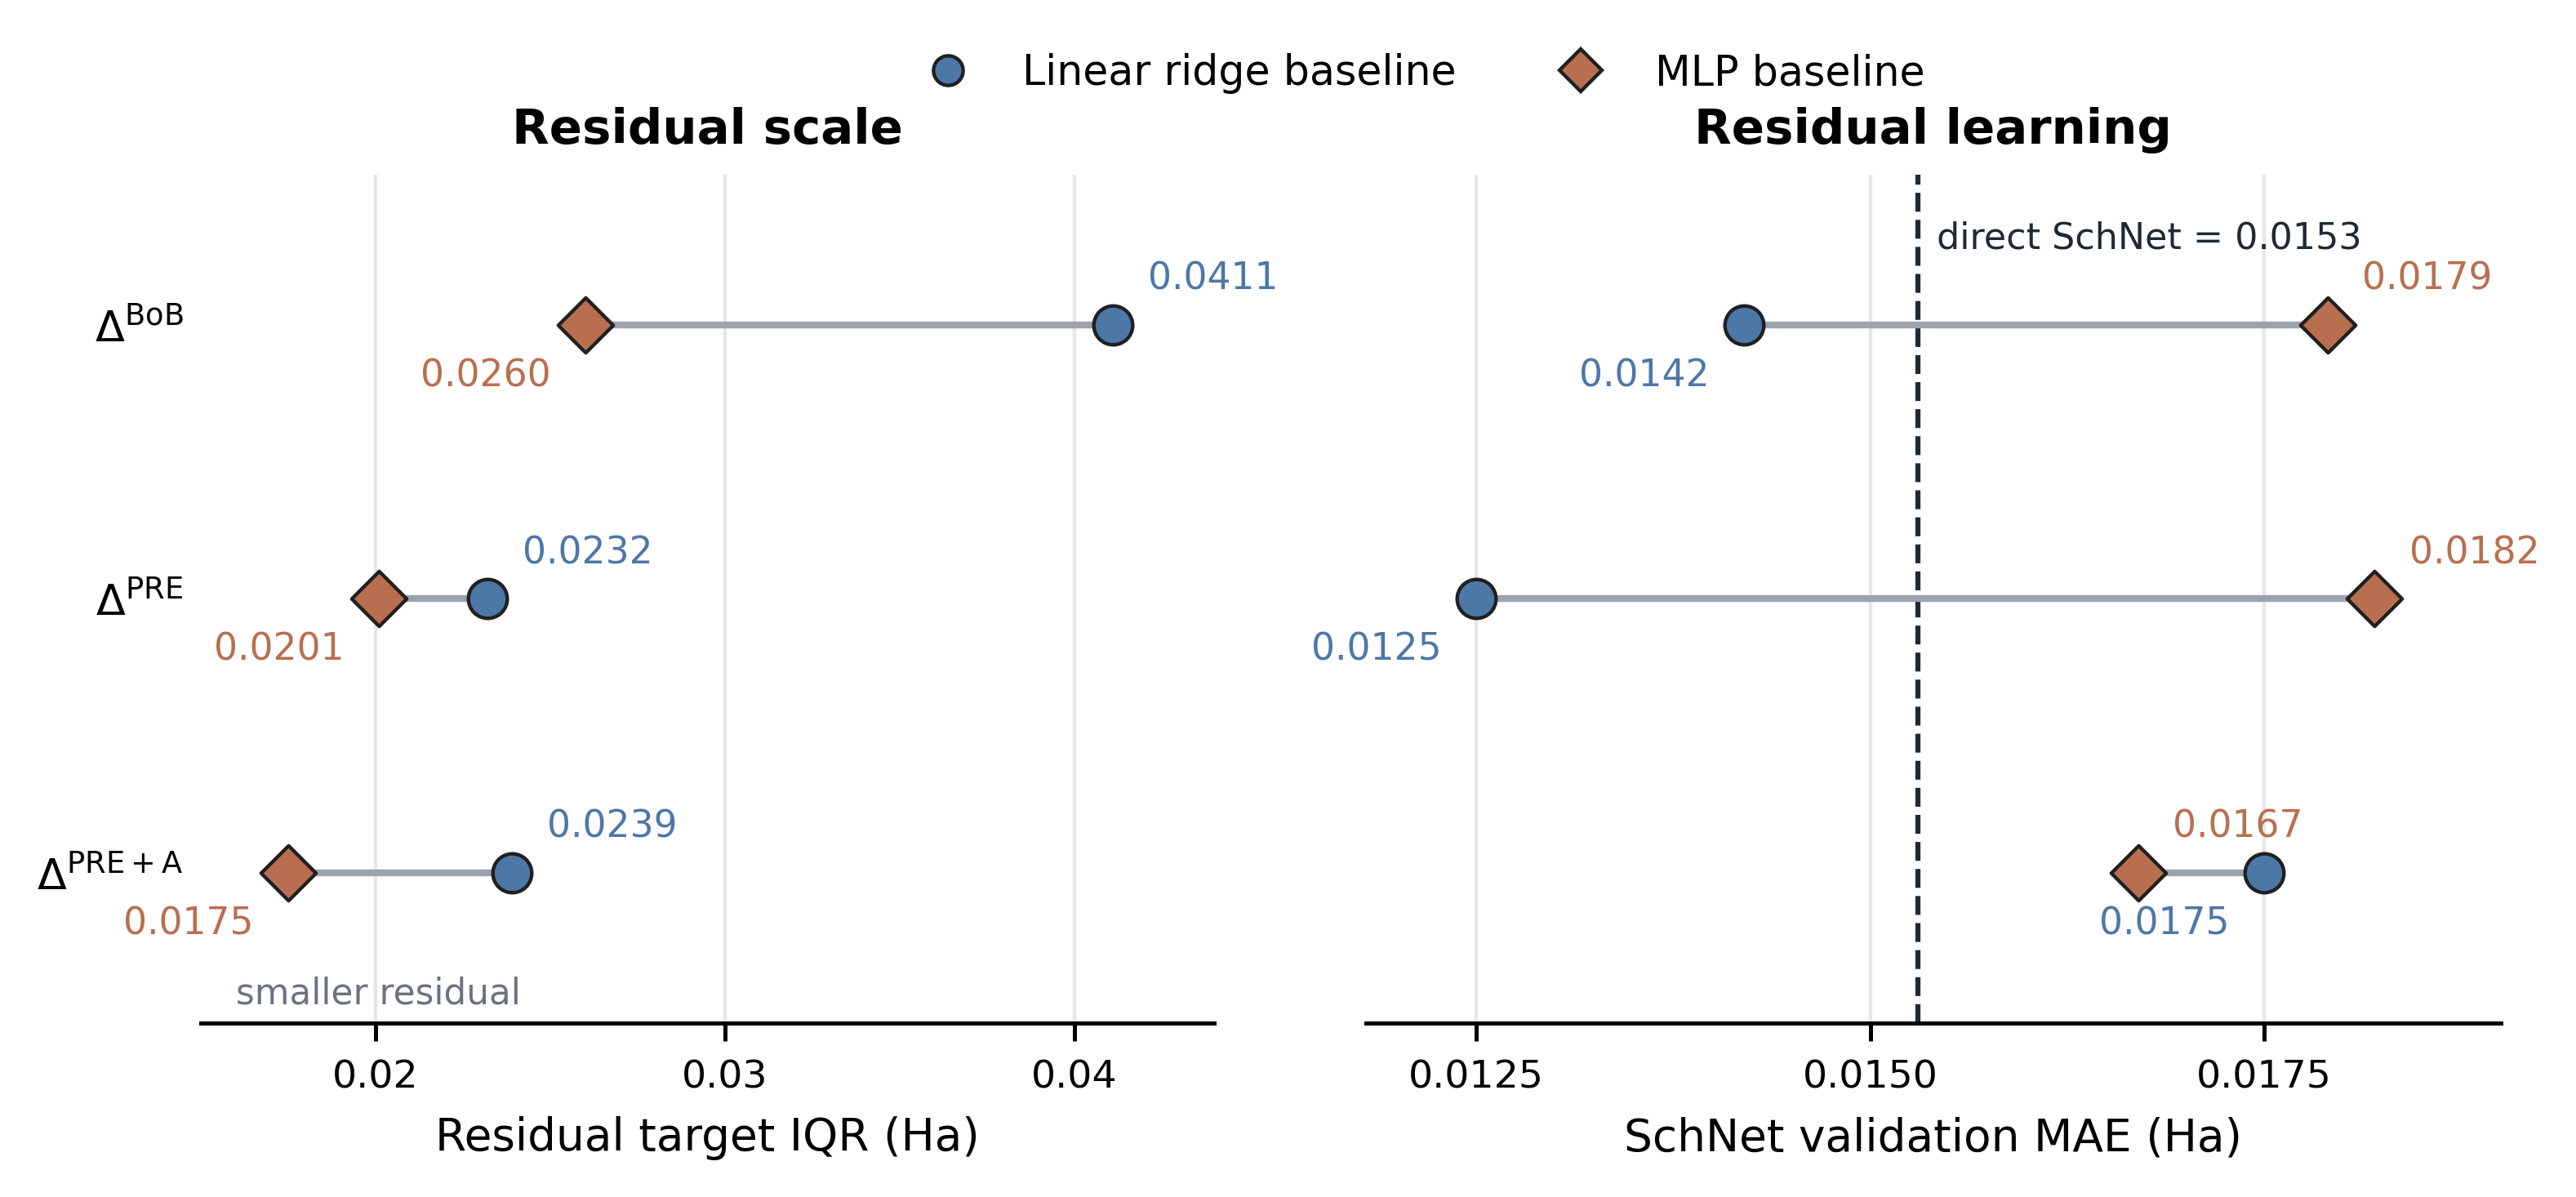
\includegraphics[width=0.95\linewidth]{schnet_val_mae_linear_vs_mlp_delta_baselines}
  \caption{SchNet analogue of the ridge-versus-MLP descriptor-baseline comparison. For each descriptor family, the left panel compares the residual IQR left by a linear ridge baseline and an MLP baseline, while the right panel shows the reconstructed SchNet validation MAE after training on the corresponding residual target. The dashed line marks direct SchNet training on \(E_{\rm ref,BoE}\) without residualization. As in GemNet, the MLP baselines leave smaller central residual scales, but they worsen SchNet validation MAE for BoB and PRE; PRE+A shows a small improvement but remains worse than direct SchNet training.}
  \label{fig:s5-schnet-linear-vs-mlp-delta-baselines}
\end{figure}

\clearpage

\section*{Supplementary Tables}

Tables~S1--S3 collect numerical diagnostics used to support the figure-level conclusions. They are intended as robustness and reproducibility summaries rather than additional design rules.

\begin{table}[H]
  \centering
  \scriptsize
  \setlength{\tabcolsep}{3pt}
  \caption{Alternative target scale, scale-normalized roughness, and residual-learning diagnostics for the \(E_{\rm ref,BoE}\) target panel. Variance and IQR quantify target scale on the tmQM validation split. \(D_{\rm var}\) denotes graph Dirichlet roughness normalized by target variance, and \(D_{\rm IQR}\) denotes the analogous roughness normalized by IQR scale. These values use the earlier raw-feature neighborhood diagnostics: GemNet roughness is measured in PRE+A space, and SchNet roughness is measured in PRE space. MAEs are reconstructed validation errors on the \(E_{\rm ref,BoE}\) scale.}
  \label{tab:target-scale-roughness-diagnostics}
  \begin{tabular}{lrrrrrrrr}
    \toprule
    Target &
    Variance &
    IQR &
    \shortstack{PRE+A\\\(D_{\rm var}\)} &
    \shortstack{PRE+A\\\(D_{\rm IQR}\)} &
    \shortstack{GemNet\\MAE} &
    \shortstack{PRE\\\(D_{\rm var}\)} &
    \shortstack{PRE\\\(D_{\rm IQR}\)} &
    \shortstack{SchNet\\MAE} \\
    \midrule
    \(E_{\rm ref,BoE}\) & 0.0084 & 0.0848 & 1.50 & 1.76 & 0.0101 & 1.36 & 1.60 & 0.0153 \\
    \(\Delta^{\rm xTB}\) & 0.0025 & 0.0503 & 1.47 & 1.47 & 0.0064 & 1.34 & 1.33 & 0.0093 \\
    \(\Delta^{\rm BoB}\) & 0.0020 & 0.0254 & 1.58 & 4.91 & 0.0174 & 1.50 & 4.68 & 0.0179 \\
    \(\Delta^{\rm PRE}\) & 0.0031 & 0.0199 & 1.58 & 12.32 & 0.0181 & 1.68 & 13.08 & 0.0182 \\
    \(\Delta^{\rm PRE+A}\) & 0.0048 & 0.0172 & 1.69 & 27.46 & 0.0168 & 1.65 & 26.80 & 0.0167 \\
    \bottomrule
  \end{tabular}
\end{table}

Table~S1 reports alternative roughness normalizations to make clear that the numerical value of a roughness score depends on the chosen feature space and scale normalization. These values are used as robustness diagnostics rather than as the primary metric in the main text.

\begin{table}[H]
  \centering
  \small
  \setlength{\tabcolsep}{7pt}
  \caption{Ridge and MLP versions of descriptor residual targets. Values are computed on the tmQM validation split after applying the shared filtered mask used for the residual-scale comparison. IQR and variance describe the scale of each residual target. GemNet and SchNet MAEs are reconstructed validation errors on the \(E_{\rm ref,BoE}\) scale after training on each residual target; equivalently, they are the residual-target MAEs.}
  \label{tab:linear-vs-mlp-residuals}
  \begin{tabular}{llrrrr}
    \toprule
    Target &
    Fit &
    IQR &
    Variance &
    \shortstack{GemNet\\MAE} &
    \shortstack{SchNet\\MAE} \\
    \midrule
    \(\Delta^{\rm xTB}\) & xTB & 0.0508 & 0.00245 & 0.0064 & 0.0093 \\
    \midrule
    \(\Delta^{\rm BoB}\) & Ridge & 0.0411 & 0.00190 & 0.0108 & 0.0142 \\
    \(\Delta^{\rm MLP-BoB}\) & MLP & 0.0260 & 0.00144 & 0.0174 & 0.0179 \\
    \(\Delta^{\rm PRE}\) & Ridge & 0.0232 & 0.00064 & 0.0123 & 0.0125 \\
    \(\Delta^{\rm MLP-PRE}\) & MLP & 0.0201 & 0.00108 & 0.0181 & 0.0182 \\
    \(\Delta^{\rm PRE+A}\) & Ridge & 0.0239 & 0.00087 & 0.0165 & 0.0175 \\
    \(\Delta^{\rm MLP-PRE+A}\) & MLP & 0.0175 & 0.00084 & 0.0168 & 0.0167 \\
    \bottomrule
  \end{tabular}
\end{table}

Table~S2 provides the numerical values underlying the ridge-versus-MLP controls in Figure~6 and Figure~S5. The table is included to separate target-scale effects, measured by IQR and variance, from the reconstructed residual-learning MAEs.

\clearpage

\begin{table}[H]
  \centering
  \scriptsize
  \setlength{\tabcolsep}{4pt}
  \caption{QM9 transfer performance after mean-shift calibration. Models are trained on tmQM and evaluated on QM9 against \(E_{\rm ref,BoE}\). Each stacked prediction is reconstructed as baseline plus GNN-predicted residual. Mean-shift calibration removes a single constant bias before computing errors; it does not change the relative ordering or scatter of the predictions.}
  \label{tab:qm9-transfer-mean-shift}
  \begin{tabular}{lllrrrr}
    \toprule
    GNN &
    Prediction &
    Source &
    \(n\) &
    \shortstack{MAE\\(Ha)} &
    \shortstack{RMSE\\(Ha)} &
    \(R^2\) \\
    \midrule
    GemNet & direct \(E_{\rm ref,BoE}\) & direct & 130807 & 0.0156 & 0.0294 & 0.673 \\
    GemNet & \(xTB+\Delta^{\rm xTB}\) & xTB & 130807 & 0.0062 & 0.0086 & 0.972 \\
    GemNet & BoB+\(\Delta^{\rm BoB}\) & Ridge & 128988 & 0.0189 & 0.0332 & 0.576 \\
    GemNet & PRE+\(\Delta^{\rm PRE}\) & Ridge & 130807 & 0.0332 & 0.0631 & -0.499 \\
    GemNet & PRE+A+\(\Delta^{\rm PRE+A}\) & Ridge & 128988 & 0.0348 & 0.0733 & -1.067 \\
    GemNet & MLP-BoB+\(\Delta^{\rm MLP-BoB}\) & MLP & 130807 & 0.0301 & 0.0429 & 0.307 \\
    GemNet & MLP-PRE+\(\Delta^{\rm MLP-PRE}\) & MLP & 128988 & 0.0598 & 0.1075 & -3.444 \\
    GemNet & MLP-PRE+A+\(\Delta^{\rm MLP-PRE+A}\) & MLP & 128988 & 0.0700 & 0.1284 & -5.343 \\
    \midrule
    SchNet & direct \(E_{\rm ref,BoE}\) & direct & 130807 & 0.0138 & 0.0265 & 0.736 \\
    SchNet & \(xTB+\Delta^{\rm xTB}\) & xTB & 130807 & 0.0070 & 0.0099 & 0.963 \\
    SchNet & BoB+\(\Delta^{\rm BoB}\) & Ridge & 128988 & 0.0440 & 0.0594 & -0.357 \\
    SchNet & PRE+\(\Delta^{\rm PRE}\) & Ridge & 130807 & 0.0533 & 0.0752 & -1.131 \\
    SchNet & PRE+A+\(\Delta^{\rm PRE+A}\) & Ridge & 128988 & 0.0404 & 0.0792 & -1.412 \\
    SchNet & MLP-BoB+\(\Delta^{\rm MLP-BoB}\) & MLP & 130807 & 0.0279 & 0.0397 & 0.407 \\
    SchNet & MLP-PRE+\(\Delta^{\rm MLP-PRE}\) & MLP & 128988 & 0.0601 & 0.1071 & -3.410 \\
    SchNet & MLP-PRE+A+\(\Delta^{\rm MLP-PRE+A}\) & MLP & 128988 & 0.0704 & 0.1287 & -5.377 \\
    \bottomrule
  \end{tabular}
\end{table}

\end{document}
